%%%%%%%%%%%%%%%%%%%%%%%%%%%%%%%%%%%%%%%%%%%%%%%%%%%%%%%%%%%
% --------------------------------------------------------
% Tau
% LaTeX Template
% Version 2.4.4 (28/02/2025)
%
% Author: 
% Guillermo Jimenez (memo.notess1@gmail.com)
% 
% License:
% Creative Commons CC BY 4.0
% --------------------------------------------------------
%%%%%%%%%%%%%%%%%%%%%%%%%%%%%%%%%%%%%%%%%%%%%%%%%%%%%%%%%%%

\documentclass[10pt,a4paper,twocolumn,twoside]{tau-class/tau}
\usepackage[english]{babel}

%% Only uncomment this if you have spanish language installed and want to use it
%% \usepackage[spanish,es-nodecimaldot,es-noindentfirst]{babel} 

%% Draft watermark
% \usepackage{draftwatermark}

%----------------------------------------------------------
% TITLE
%----------------------------------------------------------

\journalname{ELL201 Sem-2 2024-25 Project Report}
\title{CPLD Maths Game using Verilog}

%----------------------------------------------------------
% AUTHORS, AFFILIATIONS AND PROFESSOR
%----------------------------------------------------------


\author[a]{Arnav Singh}
\author[b]{Lakshya Bhatnagar}
\author[c]{Mahesh Pareek}
\author[d]{Arnav Panjla}

%----------------------------------------------------------

\affil[a]{Arnav Singh, 2023EE10968}
\affil[b]{Lakshya Bhatnagar, 2023AM10945}
\affil[c]{Mahesh Pareek, 2023MT10586}
\affil[d]{Arnav Panjla, 2023EE10978}

\professor{\textbf{Prof. Dhiman Malik} \\ \textbf{TA:} Chithambara J}

%----------------------------------------------------------
% FOOTER INFORMATION
%----------------------------------------------------------

\institution{Indian isntitute of technology, Delhi}
\theday{April 29, 2025}
\course{ELL201 Sem-2 2024-25 Project}

%----------------------------------------------------------
% ABSTRACT AND KEYWORDS
%----------------------------------------------------------
\begin{abstract}    
    This project presents the design and implementation of a memory-based arithmetic game on the MAX3000A CPLD using Verilog HDL. The system operates at a 1Hz clock rate and guides players through phases of random number display, sum calculation, input validation, and feedback through LEDs. A dedicated binary-to-BCD module ensures proper formatting for the 7-segment displays. This project reinforces concepts of sequential logic, finite state machines, and modular Verilog design in a real-world CPLD application.
\end{abstract}

%----------------------------------------------------------

\keywords{CPLD, Verilog, Memory Game, Arithmetic Game, LFSR, BCD Conversion}

%----------------------------------------------------------

\begin{document}
		
    \maketitle 
    \thispagestyle{firststyle} 
    \tauabstract 
    % \tableofcontents
    % \linenumbers 
    
%----------------------------------------------------------

\section{Introduction}

    \taustart{T}his project implements a memory-based arithmetic game on the MAX3000A CPLD using Verilog HDL. The system operates on a 1Hz clock, with each game cycle divided into five distinct phases:
    
    \begin{enumerate}
        \item A 5-bit Linear Feedback Shift Register (LFSR) generates pseudo-random numbers, which are displayed one at a time and internally summed.
        \item After displaying the numbers, the screen is cleared to allow the player to input their calculated sum using the onboard switches.
        \item The system then displays the correct sum and compares it to the player's input.
        \item LED indicators provide immediate feedback, showing success or failure through predefined light patterns.
        \item Finally, the system resets automatically to begin a new game round.
    \end{enumerate}

A separate \texttt{binary\_to\_bcd} module handles binary to BCD conversion, enabling correct representation on 7-segment displays.
	
\section{Motivation}

    The goal of this project is to practically apply concepts of Verilog programming, sequential digital design, and modular circuit development on CPLDs. By integrating a memory challenge with arithmetic operations, the project not only reinforces theoretical knowledge but also develops skills related to finite state machines, random number generation using LFSRs, and binary-BCD conversions essential for digital display systems.
    
\section{Implementation Methodology}

    \subsection{Pin Mapping}
    
    The following table summarizes the pin configuration used for interfacing the CPLD with switches, LEDs, 7-segment display outputs, and the clock:

    \begin{figure}[h!]
        \centering
        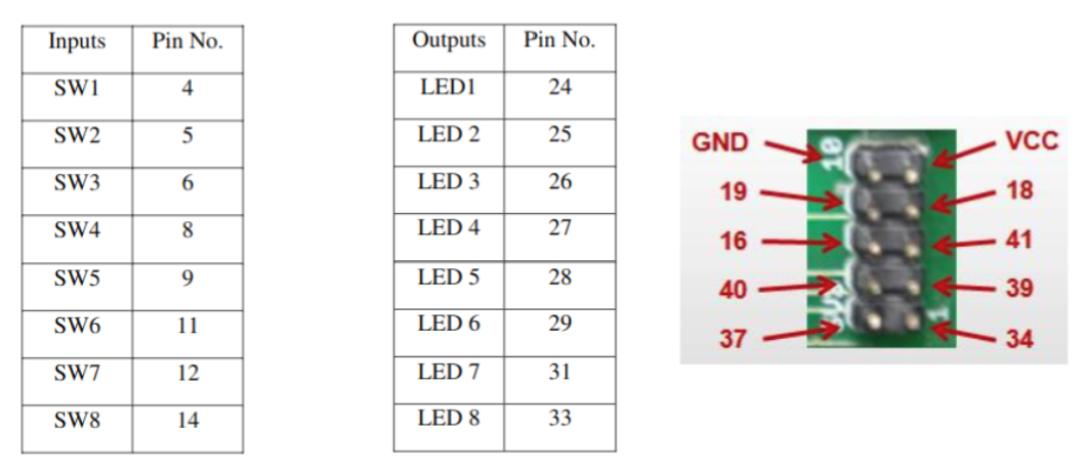
\includegraphics[width=0.52\textwidth]{figures/cpld_pinout.png}
        \caption{MAX3000A pinout for reference}
        \label{fig:circuitdiagram}
    \end{figure}

    \begin{table}[h!]
        \centering
        \begin{tabular}{|c|c|l|}
            \hline
            \textbf{Signal} & \textbf{Pin} & \textbf{Description} \\
            \hline
            clk & 43 & Global clock input (1Hz) \\
            o\_clk & 24 & Debugging clock output \\
            \hline
            bcd\_tens[3] & 34 & BCD tens place output (MSB) \\
            bcd\_tens[2] & 39 & BCD tens place output \\
            bcd\_tens[1] & 41 & BCD tens place output \\
            bcd\_tens[0] & 18 & BCD tens place output (LSB) \\
            bcd\_units[3] & 37 & BCD units place output (MSB) \\
            bcd\_units[2] & 40 & BCD units place output \\
            bcd\_units[1] & 16 & BCD units place output \\
            bcd\_units[0] & 19 & BCD units place output (LSB) \\
            \hline
            switch[7] (rst) & 14 & Reset signal input \\
            switch[6] & 12 & Switch input (bit 6) \\
            switch[5] & 11 & Switch input (bit 5) \\
            switch[4] & 9  & Switch input (bit 4) \\
            switch[3] & 8  & Switch input (bit 3) \\
            switch[2] & 6  & Switch input (bit 2) \\
            switch[1] & 5  & Switch input (bit 1) \\
            switch[0] & 4  & Switch input (bit 0) \\
            \hline
            led[6] & 33 & LED indicator (MSB) \\
            led[5] & 31 & LED indicator \\
            led[4] & 29 & LED indicator \\
            led[3] & 28 & LED indicator \\
            led[2] & 27 & LED indicator \\
            led[1] & 26 & LED indicator \\
            led[0] & 25 & LED indicator (LSB) \\
            \hline
        \end{tabular}
        \caption{Pin Mapping of MAX3000A as done in software}
        \label{tab:pinmapping}
    \end{table}
    
    \subsection{Truth Table}
    
    The truth table below outlines the system behavior during various phases of the game based on the cycle counter value:
    \vspace{15pt}
    \\
    Note - all the data are taken when seed phrase is 10101, for other seed the value will be different.

    \begin{table*}[tp]
        \centering
        \begin{tabular}{|c|c|c|c|}
            \hline
            \textbf{Cycle Counter} & \textbf{Action} & \textbf{Display Output} & \textbf{LED Status} \\
            \hline
            0-3 & Generate random number (LFSR) & Random value & Reflect LFSR value (padded) \\
            4 & Clear display & 0 & OFF \\
            5-10 & Accept user input via switches & Switch value & OFF \\
            11-12 & Display correct answer & Sum modulo 100 & LEDs ON (success or pattern) \\
            13-14 & Hold result display & Sum modulo 100 & LEDs remain in previous state \\
            15 & Reset game & 0 & LEDs ON \\
            \hline
        \end{tabular}
        \caption{Truth Table for Game Phases}
        \label{tab:truthtable}
    \end{table*}
	
    \subsection{Circuit Diagram}
    
    The circuit diagram is provided below:
    
    \begin{figure}[h!]
        \centering
        % 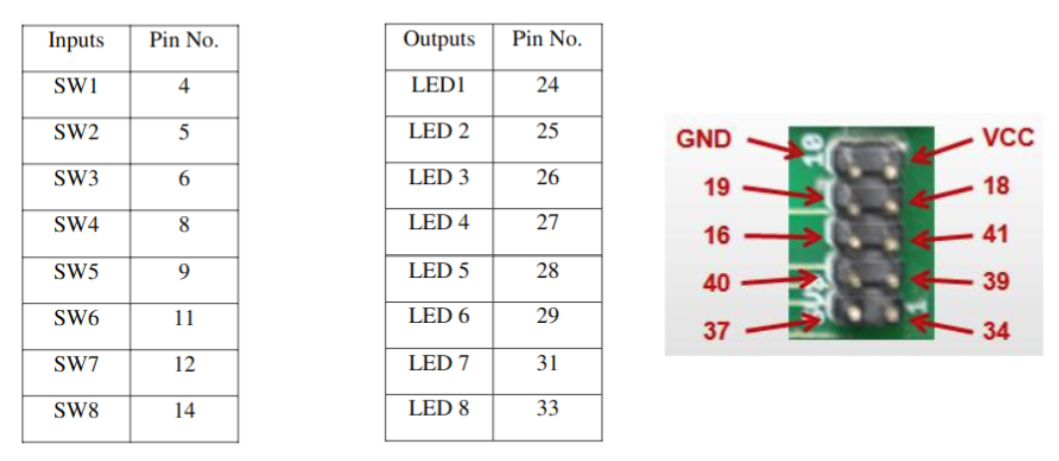
\includegraphics[width=0.8\textwidth]{images/IO mapping.png}
        \caption{CPLD Maths Game Circuit Diagram and IO Mapping}
        \label{fig:circuitdiagram}
    \end{figure}

\section{Tables and figures}

    \subsection{Tables}
	
        Table \ref{tab:table} shows an example table. The \verb|\tabletext{}| is used to add notes to tables easily. 
    		
        \begin{table}[H]
            \centering
            \caption{Astronomical Object Data}
            \label{tab:table}
            \begin{tabular}{ll}
                \toprule
                \textbf{Object} & \textbf{Distance (Light Years)} \\
                \midrule
                Alpha Centauri & 4.37 \\
                Betelgeuse & 642.5 \\
                Andromeda Galaxy & 2.537 million \\
                \bottomrule   
            \end{tabular}
			
            \tabletext{Note: The table contains data of some famous celestial objects.}
			
        \end{table}

    \subsection{Figures}
		
    	Fig. \ref{fig:figure} shows an example figure.
    		
    	\begin{figure}[H]
    		\centering
    		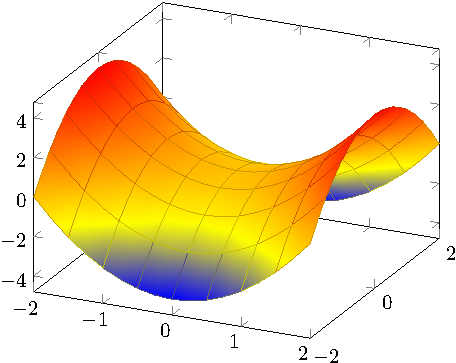
\includegraphics[width=0.75\columnwidth]{Example.pdf}
    		\caption{Example figure obtained from PGFPlots \cite{PFGPlots}.}
    		\label{fig:figure}
    	\end{figure}
		
        Fig. \ref{fig:examplefloat} shows an example of two figures that covers the width of the page. It can be placed at the top or bottom of the page. The space between the figures can also be changed using the \verb|\hspace{Xpt}| command.
		
        \begin{figure*}[tp] % t for position at the top of the current page; b for position at the bottom; p for new page
		\centering
		  \begin{subfigure}[b]{0.38\linewidth} % Fig (a)
			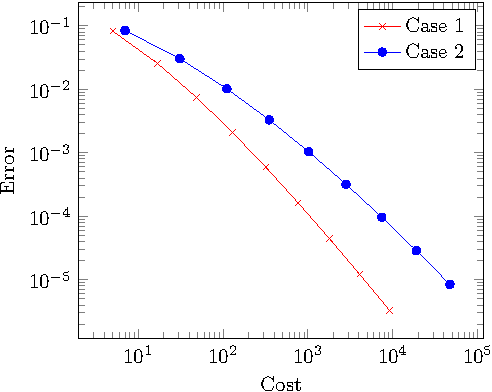
\includegraphics[width=\linewidth]{Example2.pdf}
			\caption{Example left figure.}
			\label{fig:figa}
		\end{subfigure}
			\hspace{20pt}   % Space between the figures
		\begin{subfigure}[b]{0.375\linewidth} % Fig (b)
			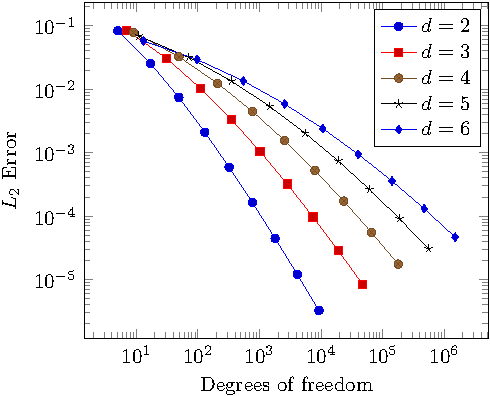
\includegraphics[width=\linewidth]{Example3.pdf}
			\caption{Example right figure.}
			\label{fig:figb}
		\end{subfigure}
		\caption{Example figure that covers the width of the page obtained from PGFPlots \cite{PFGPlots}.}
		\label{fig:examplefloat}
	\end{figure*}
		
\section{Tau packages}

    \subsection{Tauenvs}
	
        This template has its own environment package \textit{tauenvs.sty} designed to enhance the presentation of the document. Among these custom environments are \textit{tauenv}, \textit{info} and \textit{note}.
		
        There are two environments which have a predefined title. These can be included by the command \verb|\begin{note}| and \verb|\begin{info}|. All the environments have the same style.
			
        An example using the tau environment is shown below.
		
    	\begin{tauenv}[frametitle=Environment with custom title]
            This is an example of the custom title environment. To add a title type \verb|[frametitle=Your title]| next to the beginning of the environment (as shown in this example).
    	\end{tauenv}
		
        Tauenv is the only environment that you can customize its title. On the other hand, info and note adapt their title to Spanish automatically when this language package is defined.
		
    \subsection{Taubabel}

        In previous versions, we included a package called \textit{taubabel}, which have all the commands that automatically translate from English to Spanish when this language package is defined. 
        
        By default, tau displays its content in English. However, at the beginning of the document you will find a recommendation when writing in Spanish. 
		
        \textit{Note:} You may modify this package if you want to use other language than English or Spanish. This will make easier to translate the document without having to modify the class document.
		
\section{Equation}

    Equation \ref{ec:equation}, shows the Schrödinger equation as an example. 
	\begin{equation} \label{ec:equation}
		\frac{\hbar^2}{2m}\nabla^2\Psi + V(\mathbf{r})\Psi = -i\hbar \frac{\partial\Psi}{\partial t}
	\end{equation} 
    The \textit{amssymb} package was not necessary to include, because stix2 font incorporates mathematical symbols for writing quality equations. In case you choose another font, uncomment this package in tau-class/tau.cls/math packages.
	
    If you want to change the values that adjust the spacing above and below the equations, play with \verb|\setlength{\eqskip}{8pt}| value until the preferred spacing is set.
	
\section{Adding codes}
	
    This class\footnote{Hello there! I am a footnote :)} includes the \textit{listings} package, which offers customized features for adding codes in \LaTeX\ documents specifically for C, C++, \LaTeX\ and Matlab. 
	
    You can customize the format in tau-class/tau.cls/listings style.
	
    \lstinputlisting[caption=Example of Matlab code., language=Matlab,label=code]{example.m}
	
    If line numbering is defined at the beginning of the document, I recommend placing the command \verb|\nolinenumbers| at the start and \verb|\linenumbers| at the end of the code. 
    
    This will temporarily remove line numbering and the code will look better.
	


\printbibliography

%----------------------------------------------------------

\end{document}